\section{Results}

\subsection{Theoretical derivations}
In this section we summarise the equations used in our numerical implementation and present the background evolution of the inflaton in the simplified decoupled limit. Consider the Lagrangian density \cite{Apostolos}

\begin{equation}
    \mathcal{L} = \frac{1}{2} \nabla_{\mu} \phi \nabla^{\mu} \phi + \nabla_{\mu} \psi^* \nabla^{\mu} \psi - V(\phi) - \frac{1}{2} m_{\psi}^2(\phi) |\psi|^2 - \frac{\lambda}{4} |\psi|^4 - \frac{\lambda}{4}f^4,
\end{equation}
with the mass term

\begin{equation}
    m_{\psi}^2(\phi) = g^2 (\phi - \phi_{SBP})^2 - \lambda f^2,
\end{equation}
where the $\nabla_{\mu}$ denotes the covariant derivative, $\lambda$, $g$ and $f$ are free parameters. In particular $\lambda$ and $g$ are coupling constants. Here $f^4$ is the constant vacuum energy expectation value, in order to normalise the potential so that the true vacuum energy is zero \cite{dimopoulos2019quintessential}. In addition, $\phi$ is the inflaton field and $\psi$ is complex spin-0 scalar field. Finally, $\phi_{SBP}$ is the inflaton value at the symmetry-breaking point. 

% After the usual process of varying the fields we obtain the equation of motion for $\psi$

% \begin{equation}
%     \ddot{\psi} + 3H \dot{\psi} - \frac{1}{a^2} \nabla^2 \psi + \frac{\delta \mathcal{V}}{\delta \psi^{\dag}} = - \frac{\delta V}{\delta \psi^{\dag}}
% \end{equation}

% Where $\mathcal{V}$ is the potential energy density and $V$ was added as an external CP-violating potential. 

We can compute the particle number density, using Noether current, to be

\begin{equation}
    \dot{n} + 3H n = 2 \mathrm{Im} \left( \psi \frac{\delta V}{\delta \psi^{\dag}} \right)
\end{equation}
Next, we can decompose the complex scalar field in the polar form
\begin{equation}
    \psi(x,t) = \frac{1}{\sqrt{2}} \chi(x,t) e^{i \theta(x,t)},
\end{equation}
here $\chi$ is the radial (amplitude) mode and $\theta$ is the angular (phase) mode. Thus we obtain the following equations of motion

\begin{align}
\ddot{\chi} + 3H\dot{\chi}
-\left[\dot{\theta}^{\,2}-\frac{1}{a^{2}}(\nabla\theta)^{2}\right]\chi
+\frac{\delta \mathcal{V}}{\delta \chi}
&= -\,\frac{\delta V}{\delta \chi},
\\[6pt]
\ddot{\theta}
+\left[3H + 2\,\partial_{0}\ln(\chi)\right]\dot{\theta}
-\frac{1}{a^{2}}\Big[\nabla^{2}\theta + 2\,\nabla\ln(\chi)\cdot\nabla\theta\Big]
&= -\,\frac{1}{\chi^{2}}\frac{\delta V}{\delta \theta}.
\end{align}
Here $V_A$ denotes the CP-violating term responsible for charge production. Similarly, we apply the decomposition to the particle number to get

\begin{equation}
\dot{n} + 3Hn
= \frac{1}{a^{2}}\,\nabla\cdot\left(\chi^{2}\nabla\theta\right)
- 2\,\mathrm{Im}\!\left(\psi\,\frac{\delta V_A}{\delta\psi}\right).
\end{equation}

For computational results it is more useful to use the average, which is a typical result

\begin{equation}
\langle \dot{n} \rangle + 3H \langle n \rangle
= -2 \left\langle \mathrm{Im}\!\left(\psi\,\frac{\delta V_A}{\delta\psi}\right) \right\rangle .
\end{equation}

If we were to keep the fluctuations, we would have to replace the non-linear terms. Since in general $\chi(t)$ and $\theta(t)$ are inhomogeneous fields we can replace these terms using Hartree-Fock approximation

\begin{equation}
    \chi^3 \rightarrow 3 \langle \chi^2 \rangle \chi
\end{equation}
remember that $\phi$ depends on time and is homogeneous in space and more precisely is the expectation value, while $\chi$ and $\theta$ are inhomogeneous fields whose mean values vanish, $\langle \chi \rangle = \langle \theta \rangle = 0$, but with non-zero variance such as $\langle \chi^2 \rangle$. Taking $V(\phi) = V_0 \exp [- \kappa \exp(\frac{\phi}{b \mpl})]$, where $b = \sqrt{a}$ with $\kappa$ being a free parameter. $V_0$ can be obtained from observations. In particular, equations of motion in Fourier space can be derived

\begin{equation}
\ddot{\phi} + 3H \dot{\phi}
 - \frac{\kappa V_0}{b M_{\rm Pl}}
 \exp\!\left[\frac{\phi}{b M_{\rm Pl}} - \kappa e^{\frac{\phi}{b M_{\rm Pl}}}\right]
 + g^2 \langle \chi^2 \rangle (\phi - \phi_{\rm SBP}) = 0
\end{equation}

\begin{equation}
\ddot{\tilde{\chi}}_{\mathbf{k}} + 3H \dot{\tilde{\chi}}_{\mathbf{k}}
+ \left[
\frac{k^2}{a^2}
+ g^2 (\phi - \phi_{\rm SBP})^2
- \lambda f^2
+ 3 \lambda \langle \chi^2 \rangle + \langle \dot{\theta}^2 \rangle
+ \frac{1}{a^2} \langle (\nabla \theta)^2 \rangle
\right]
\tilde{\chi}_{\mathbf{k}} = 0
\end{equation}

\begin{equation}
\langle \chi^2 \rangle \ddot{\tilde{\theta}}_{\mathbf{k}}
+ (2 \langle \chi \dot{\chi} \rangle + 3H \langle \chi^2 \rangle) \dot{\tilde{\theta}}_{\mathbf{k}}
+ \frac{k^2}{a^2} \langle \chi^2 \rangle \tilde{\theta}_{\mathbf{k}} = 0
\end{equation}
where the averages are

\begin{equation}
\langle \chi^2 \rangle
= \int_{\mathbb{R}^3} \frac{d^3 p}{(2\pi)^3}
\left[ |\tilde{\chi}_{\mathbf{p}}(t)|^2 + \text{2PI-corrections} \right]
\end{equation}

\begin{equation}
\langle \dot{\theta}^2 \rangle
= \int_{\mathbb{R}^3} \frac{d^3 p}{(2\pi)^3}
\left[ |\dot{\tilde{\theta}}_{\mathbf{p}}(t)|^2 + \text{2PI-corrections} \right]
\end{equation}
here the 2PI-corrections stand for two particle irreducable corrections. These corrections account for backreaction, rescattering and thermalisation effects, which become important during preheating, especially when produced fluctuations grow large.

The shape of the potential is very important and is plotted as follows:

% \begin{center}
%     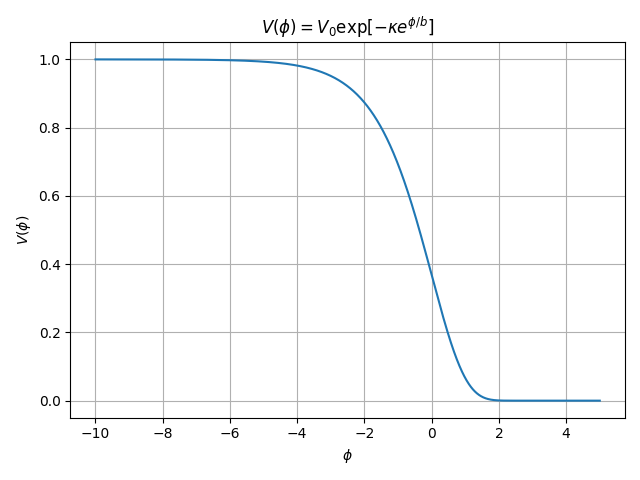
\includegraphics[width=300pt]{images/potential.png}
% \end{center}

\begin{figure}[H]
    \centering
    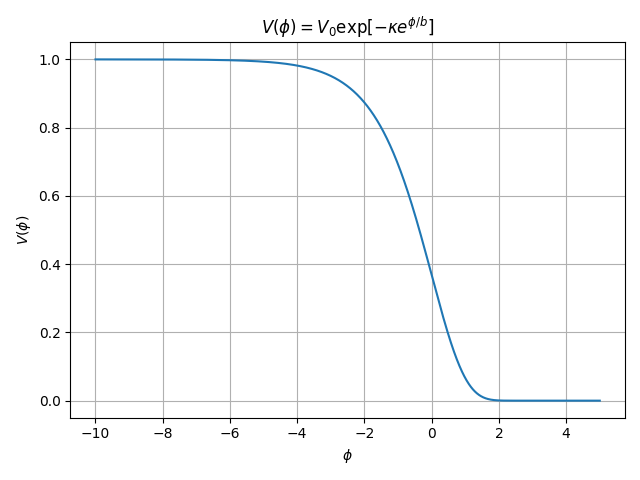
\includegraphics[width=300pt]{images/potential.png}
    \caption{Shape of the inflationary potential $V(\phi)=V_0\exp\!\left[-\kappa\exp\!\left(\phi/(bM_{\rm pl})\right)\right]$. The plot was generated in this work to illustrate the nearly flat region at small $\phi$ (supporting slow-roll inflation) followed by a rapid drop, which strongly affects the inflaton dynamics and the end of inflation.}
    \label{fig:potential}
\end{figure}


Notice that for small $\phi$, the potential is nearly flat, supporting slow-roll inflation, while at large $\phi$ it decreases rapidly, strongly affecting the end of inflation and the symmetry-breaking transition. Until it reaches some threshold and starts to rapidly fall. More importantly, this potential does not have a minimum, so an alternative mechanism of reheating is required. At around $\phi_{SBP}$, the effective mass of $\phi$ changes sign (becomes tachyonic), triggeting symmetry breaking and rapid growth. Then the inflaton can start oscillating and transfer energy to the other fields. Similar potentials, namely, exponential potential was investigated previously \cite{karvciauskas2022quintessential}, however with the release of new data, it was found that the model does not work in all regimes.

\begin{figure}[H]
    \centering
    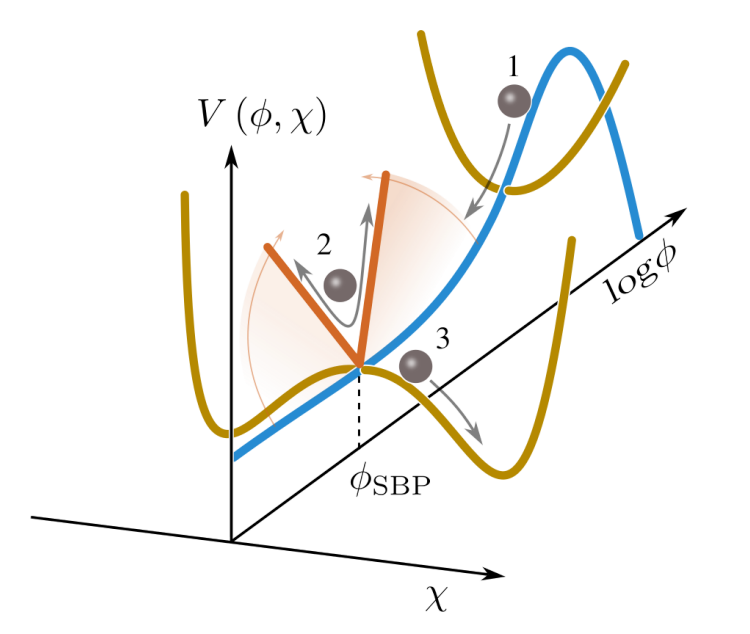
\includegraphics[width=300pt]{images/potential illustration.png}
    \caption{Illustration of the evolution of the inflaton field. After slow-roll rolling along the blue direction (stage 1), the field reaches the SBP and resonantly excites $\chi$, generating an effective linear potential and amplifying metric perturbations (stage 2). When resonance ends, the system rolls along the waterfall potential (brown) with $\phi=\phi_{\rm SBP}$. This illustration is from \cite{karciauskas2025primordial}}
    \label{fig:potential illustration}
\end{figure}

For the beginning of the project, we first take a simplified case, where we only investigate the evolution of the inflaton field. This simplification effectively describes the inflation period, during which the $\psi$ field is heavy, hence we take $\langle \chi \rangle = \langle \theta \rangle = 0$. Then the $\phi$ equations of motion are simply

\begin{equation}
    \ddot{\phi} + 3H \dot{\phi} - \frac{\kappa V_0}{b M_{\rm Pl}} \exp\!\left[\frac{\phi}{b M_{\rm Pl}} - \kappa e^{\frac{\phi}{b M_{\rm Pl}}}\right] = 0
\end{equation}
Changing the variables from time to the number of e-folds 

\begin{equation}
    t \rightarrow N, \quad \text{where} \quad N = \ln a
\end{equation}

\begin{equation}
    \dot{A} = H A^{\prime} \quad \text{and} \quad \ddot{A} = H^2 A^{\prime \prime} + H^{\prime} H A^{\prime}
\end{equation}
where the primes denote derivatives with respect to $N$. Using the Klein–Gordon equation together with the Friedmann and acceleration equations, we obtain

\begin{equation}
    \phi^{\prime \prime} + \left( 3 - \frac{{\phi^{\prime}}^2}{2 \mpl^2} \right) \phi^{\prime} + \left( 3 \mpl^2 - \frac{1}{2} {\phi^{\prime}}^2 \right) \frac{V_{, \phi}}{V} = 0
\end{equation}
Another, similar trick can be used with potential

\begin{equation}
    W = \ln V \quad \Rightarrow \quad W_{, \phi} = \frac{V_{, \phi}}{V}
\end{equation}
This is especially useful, since our potential is exponential, so using $V(\phi) = V_0 \exp \left[ - \kappa e^{\frac{\phi}{b M_{\text{Pl}}}} \right]$ we get

\begin{equation}
    W = - \kappa \exp \left( \frac{\phi}{b \mpl} \right) + W_0 \quad \text{and} \quad W_{, \phi} = -\frac{\kappa}{b \mpl} \exp \left( \frac{\phi}{b \mpl} \right)
\end{equation}
where $W_0 = \ln V_0$. Furthermore by multiplying everything by $\phi^{\prime}$, then $\phi^{\prime \prime} \phi^{\prime} = \frac{1}{2} ({\phi^{\prime}}^{2})^{\prime}$ and $W_{, \phi} \phi^{\prime} = b \mpl W^{\prime}$, hence

\begin{equation}
    ({\phi^{\prime}}^{2})^{\prime} + \left( 6 - {\phi^{\prime}}^2 \right) {\phi^{\prime}}^2 + \left( 6 - {\phi^{\prime}}^2 \right) b W^{\prime} = 0
\end{equation}
where we used $\mpl = 1$. There is also the kination limit, which was discussed a bit earlier. These equations can now be numerically simulated. Before proceeding to numerical results, approximations can also be considered. As mentioned before, we can use slow roll approximation for the beginning of inflation, when potential terms dominate kinetic terms. Consider that $|\ddot{\phi} | \ll |3 H \dot{\phi}|$ and $|\ddot{\phi} \ll |V_{, \phi} (\phi)|$, so Friedmann equation simplifies to

\begin{equation}
    H^2 = \frac{V(\phi)}{3 \mpl^2}
\end{equation}
And slow-roll Klein-Gordon equation (variables depending on time) become:
\begin{equation}
    3H \dot{\phi} = - V_{, \phi}(\phi)
\end{equation}
Again, using the same change of variables $t \rightarrow N$ we have
\begin{equation}
    3H^2 \phi^{\prime} = - V_{, \phi} \quad \Rightarrow \quad \phi^{\prime} = - \mpl^2 \frac{V_{, \phi}(\phi)}{V(\phi)} = - \mpl^2 W_{, \phi}
\end{equation}
This now is easily solvable analytically, again, setting $\mpl = 1$

\begin{align*}
    N - N_0 = \int -\frac{1}{W_{, \phi}} d\phi = \int \frac{b}{\kappa} \exp \left( - \frac{\phi}{b} \right) d \phi = -\frac{b^2}{\kappa} \exp(-\frac{\phi}{b})
\end{align*}
Finally, obtaining

\begin{equation}
    \phi(N) = - b \ln \left( \frac{\kappa}{b^2} (N_0 - N) \right) = - b \ln \left( e^{-\phi_0/b} \frac{\kappa}{b^2} - N \right)
\end{equation}

This is just a simple exponential growth, which can be seen in the following figure.

% \begin{center}
%     
\includegraphics[width=300pt]{images/slowroll.png}
% \end{center}
\begin{figure}[H]
    \centering
    
\includegraphics[width=300pt]{images/slowroll.png}
    \caption{Analytic slow-roll solution $\phi(N)$ as a function of the number of e-folds $N=\ln a$ for the exponential-to-exponential potential. This curve was plotted in this work from the derived closed-form expression and demonstrates the characteristic gradual evolution of the inflaton during the slow-roll phase.}
    \label{fig:slowroll}
\end{figure}

Conversely, kination limit can also be investigated. As mentioned before, in this limit, the kinetic terms dominate. This is a simpler problem since we can neglect the potential leaving
\begin{equation}
    \phi^{\prime \prime} + \left( 3 - \frac{\phi^{\prime 2}}{2 \mpl^2} \right)\phi^{\prime} \approx 0
\end{equation}

Solving this equation gives the attractor:
\begin{equation}
    \phi(N) = \phi_* \pm \sqrt{6} (N - N_*)
\end{equation}

with $\mpl = 1$ and the star index notation meaning, that the value of the field and e-fold number is at some reference point.

\newpage

\subsection{Numerical calculations}

To solve the dynamical system numerically, the equations of motion were first
rewritten in a first-order vector form suitable for Runge-Kutta integration.
In particular, each second-order equation of the form $\ddot{x}=F(x,\dot{x},t)$
was mapped to a coupled first-order system by introducing an auxiliary variable
$v\equiv \dot{x}$, such that
\begin{equation}
    \dot{x}=v,
    \qquad
    \dot{v}=F(x,v,t).
\end{equation}
The resulting state vector is then evolved using a fixed-step fourth-order
Runge-Kutta (RK4) method.

The numerical procedure is summarized as follows:

\begin{itemize}
    \item \textbf{Initial conditions and slow-roll start.}
    Since the initial value of $\dot{\phi}$ is not specified independently, we
    initialize the inflaton dynamics in the slow-roll regime.
    Using the slow-roll approximation, we estimate $\dot{\phi}_0$ and compute
    the initial slow-roll parameter
    \begin{equation}
        \epsilon \equiv \frac{\dot{\phi}^{2}}{2H^{2}M_{\rm Pl}^{2}},
    \end{equation}
    with $M_{\rm Pl}=1$ in geometrised units. The Hubble rate is evaluated self-consistently from the Friedmann equation \ref{eq: Friedmann equation}.

    \item \textbf{Evolution until the end of inflation.}
    Starting from the slow-roll initial conditions, the full equations of motion
    are integrated forward in time (or equivalently in e-folds $N$) until inflation
    ends, defined by the condition $\epsilon=1$. The corresponding time $t_{\rm end}$
    (or $N_{\rm end}$) is recorded.

    \item \textbf{Locating the symmetry-breaking transition.}
    During the integration we identify the symmetry-breaking point by monitoring
    the model-dependent condition for the transition (e.g.\ the vanishing of an
    effective mass term or the crossing $\phi=\phi_{\rm SB}$). This defines the
    transition time $t_{\rm SB}$ (or $N_{\rm SB}$).

    \item \textbf{Restarting the integration near the transition.}
    To resolve the dynamics around symmetry breaking with improved numerical
    stability, we restart the integration at a time slightly before the transition,
    $N_{\rm start}=N_{\rm SB}-\Delta N$, with $\Delta N$ chosen to be a small number
    of e-folds. The system is then evolved through the transition and into the
    post-inflationary regime.
\end{itemize}

Finally, the implementation was designed to be modular and scalable, allowing the model parameters, initial conditions, and numerical settings (step size, stopping conditions, and diagnostics) to be modified in a straightforward way for further development and parameter scans.

The evolution of the inflaton field is as expected, a rapid growth resembling an exponential.

% \begin{center}
%     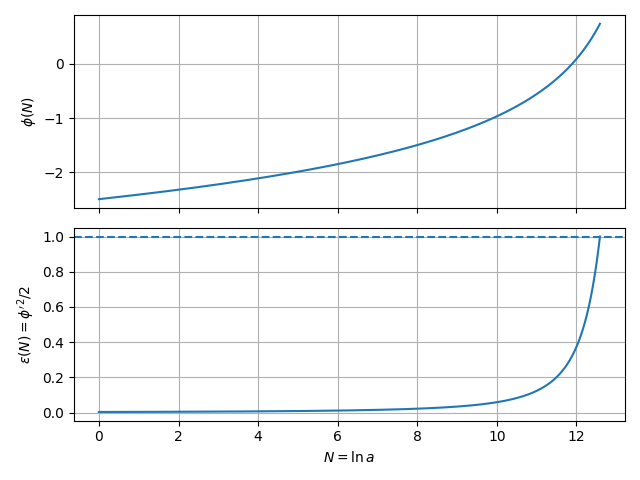
\includegraphics{images/phi evolution.png}
% \end{center}

\begin{figure}[H]
    \centering
    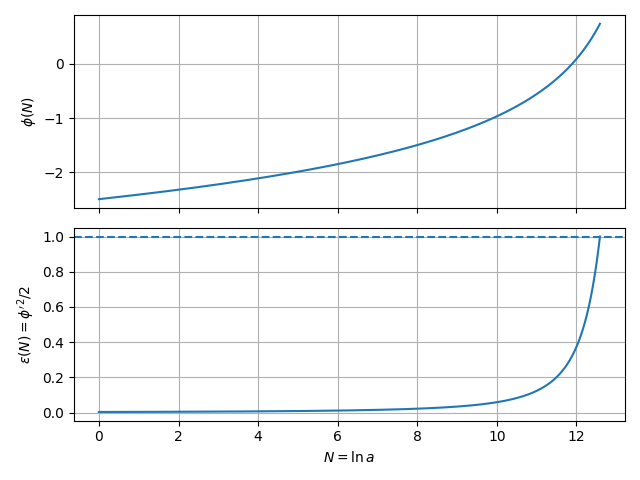
\includegraphics[width=300pt]{images/phi evolution.png}
    \caption{Numerical evolution of the inflaton field $\phi(N)$ obtained in this work using a fixed-step RK4 integrator. The solution shows the expected rapid growth in the chosen model, and inflation terminates at $N_{\rm end}\approx 12.59$ as determined by the condition $\epsilon=1$.}
    \label{fig:phievolition}
\end{figure}

In the inflaton-only approximation, the only damping is Hubble friction. Since no energy is transferred into other fields, the inflaton does not experience additional effective dissipation, and its post-inflationary evolution becomes unrealistic. $N_{\rm end} \approx 12.592333$. We verified numerical stability by repeating the integration with smaller step sizes and confirming that $N_{\rm end}$ converges. Plotting the particle number we observe a similar result as in the simplified model

% \begin{center}
%     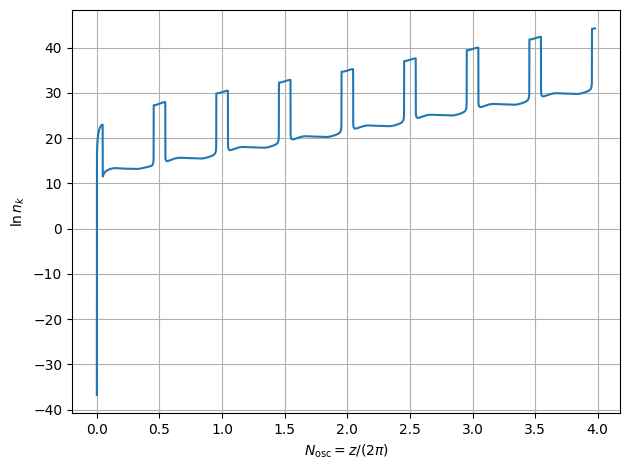
\includegraphics[width=300pt]{images/particle production phi.png}
% \end{center}

\selectlanguage{english}
\begin{figure}[H]
    \centering
    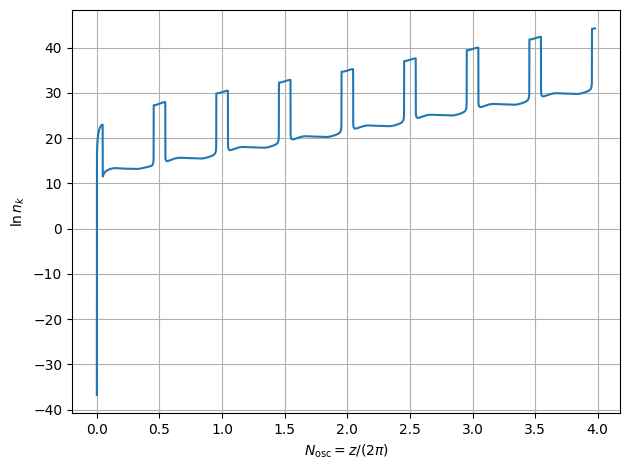
\includegraphics[width=300pt]{images/particle production phi.png}
    \caption{Comoving particle production indicator $\ln n_k$ obtained numerically in this work during the evolution of the inflaton-only system. The step-like increase with intermediate jumps is a coordinate artifact of using comoving variables; a more physical treatment including the coupled $\chi$ and $\theta$ fields would introduce backreaction and effective friction, modifying both the inflaton evolution and particle production rate.}
    \label{fig:particle_production_phi}
\end{figure}

Here we can notice a slight difference to the previous results, it is that the number of particles seems to be growing monotonically with jump-like intermediate behaviour. This, again is the consequence of the choice of coordinates. The computation of the particle number would obviously change with the introduction of $\chi$ and $\theta$. These fields would act as friction, limiting the growth of $\phi$, by converting the inflaton field energy into particle production. Note however, that the coupling is non-trivial, so further investigation must be done.

It should be noted that the numerical results presented here are just a simplified background evolution where the inflaton is evolved independently by taking $\langle \chi \rangle=\langle \theta \rangle=0$. While this approximation is sufficient for capturing the inflationary stage and determining $N_{\rm end}$, it neglects the most important reheating effects: energy transfer from $\phi$ into matter degrees of freedom, backreaction on the inflaton dynamics, and the emergence of an effective friction term sourced by particle production. Consequently, the post-inflationary evolution in the inflaton-only system is not expected to be physically realistic, since $\phi$ does not dissipate energy and its growth remains unbounded. Furthermore, the occupation number $n_k$ computed in comoving variables can exhibit non-monotonic behaviour which depends on the choice of coordinates and on the definition of the instantaneous frequency $\omega_k(t)$. Further work is required to include the $\chi$ and $\theta$ evolutions, together with the averages and PI corrections.